\documentclass[10pt]{article}

\usepackage[latin1]{inputenc}
\usepackage{amsmath, amssymb, amsfonts, amsthm}
\usepackage{upgreek}
\usepackage{amsthm}
\usepackage{fullpage}
\usepackage{graphicx}
\usepackage{cancel}
\usepackage{subfigure}
\usepackage{mathrsfs}
\usepackage{outlines}
\usepackage[font={sf,it}, labelfont={sf,bf}, labelsep=space, belowskip=5pt]{caption}
\usepackage{hyperref}
% \usepackage{minted}
\usepackage{titling}

\usepackage{fancyhdr}
\usepackage[title]{appendix}

\DeclareMathOperator{\sgn}{sgn}

\pagestyle{fancy}
\headheight 24pt
\headsep    12pt
\lhead{Material Property Design}
\rhead{\today}
\fancyfoot[C]{} % hide the default page number at the bottom
\lfoot{}
\rfoot{\thepage}
\renewcommand{\headrulewidth}{0.4pt}
\renewcommand\footrulewidth{0.4pt}
\providecommand{\abs}[1]{\lvert#1\rvert}
\providecommand{\norm}[1]{\lVert#1\rVert}
\providecommand{\dx}{\, \mathrm{d}x}
% \providecommand{\vint}[2]{\int_{#1} \! #2 \, \mathrm{d}x}
% \providecommand{\sint}[2]{\int_{\partial #1} \! #2 \, \mathrm{d}A}
\renewcommand{\div}{\nabla \cdot}
\providecommand{\shape}{\Omega(p)}
\providecommand{\mesh}{\mathcal{M}}
\providecommand{\boundary}{\partial \shape}
\providecommand{\vint}[1]{\int_{\shape} \! #1 \, \mathrm{d}x}
\providecommand{\sint}[1]{\int_{\boundary} \! #1 \, \mathrm{d}A}
\providecommand{\pder}[2]{\frac{\partial #1}{\partial #2}}
\providecommand{\tder}[2]{\frac{\mathrm{d} #1}{\mathrm{d} #2}}
\providecommand{\evalat}[2]{\left.#1\right|_{#2}}
\newcommand{\defeq}{\vcentcolon=}
\newtheorem{lemma}{Lemma}

\makeatletter
\usepackage{mathtools}
\newcases{mycases}{\quad}{%
  \hfil$\m@th\displaystyle{##}$}{$\m@th\displaystyle{##}$\hfil}{\lbrace}{.}
\makeatother

\setlength{\droptitle}{-50pt}
\title{Approach to Material Property Design}
\author{}
% Move date up over where author would be...
\date{\vspace{-24pt} \today}

% BEGIN DOCUMENT
\begin{document}
\maketitle
We outline the basic approach and tools needed to achieve spatially varying
material properties on a single material printer via periodic, patterned
microstructures. We assume for now that we are given a coarse volume mesh,
$\mesh_c$, and that each element has been assigned an elasticity tensor or
material parameters. Ideally, each of these tensors lies in the space of
homogenized tensors spanned by our chosen patterns (this could be enforced by
the tool/optimization used to assign material properties). Our goal is to create
a fine-scale volume mesh, $\mesh_f$, filled with the printer's single,
homogeneous material so that the homogenized behavior of $\mesh_f \cap e$
approximates $e$'s input elasticity tensor for all coarse volume elements $e \in
\mesh_c$.
\section{Overview}
 The general approach is as follows:
\begin{enumerate}
    \setcounter{enumi}{-1}
    \item Read in the target material properties, $m_e$, for each $e \in
        \mesh_c$. These could be in the form of
        \label{step:read}
        \begin{enumerate}
            \item ``painted'' elasticity tensors from a library we know our
                patterns can approximate;
            \item elasticity tensors fit to object deformation measurements (e.g.
                  Matusik's ``shoe paper'', \cite{Bickel2010}); or
            \item elasticity tensors optimizing some objective (minimum
                  compliance, desired deformation, desired force
                  feedback).
        \end{enumerate}
    \item Fit pattern parameters. For each element $e \in \mesh_c$, invert the
        pattern parameters $\to$ material properties map to find parameters,
        $p_e$, for the periodic pattern closest to achieving the desired
        properties.
        \label{step:fit}
        \begin{enumerate}
            \item Use a precomputed pattern parameter to material properties
                lookup table built for our patterns to interpolate an
                approximate inverse. This table could be built by sampling an
                ``$\epsilon \to 0$'' formula, e.g. for sequential laminates
                \cite{allaire2002shape}, or by numerical homogenization \`a la
                \cite{Kharevych2009}.
            \item If we have an explicit ``$\epsilon \to 0$'' formula, run some
                iterations of Newton's method to improve the inverse.
        \end{enumerate}
        Notice that here we are taking advantage of Theorem 2.1.2 from
        \cite{allaire2002shape} to work pointwise; it says that a homogenized
        material field is valid/achievable if and only if its tensor value at
        every point is an elasticity tensor obtained by periodic homogenization.
    \item Generate a printable, fine-scale mesh, $\mesh_f$. Because patterns
        need to ``connect'' across coarse element boundaries, we cannot operate
        on each coarse element in isolation.
        \label{step:mesh}
        \begin{enumerate}
            \item Choose a length scale, $\epsilon$, (periodic cell size) based
                on printer resolution and printability concerns (thin features,
                etc.).
            \item Subdivide each $e \in \mesh_c$ into cells of this size,
                filling each with a mesh of the periodic pattern specified by
                $p_e$.
            \item Stitch together the microstructure cell meshes (see Section
                \ref{sec:gen_connect}).
        \end{enumerate}
    \item Fabricate $\mesh_f$.
    \label{step:fabricate}
\end{enumerate}

\section{Validation}
Each stage of the pipeline will introduce errors, and it will be important to
measure these errors individually.

From this write-up's perspective, step \ref{step:read} gives the ground truth:
the final, fabricated object better behave like a FEM simulation of $\mesh_c$.
However, if/when the scope of our project expands to include
compliance/deformation optimization or object duplication, we will need to see
how much this simulation differs from the desired result.

Step \ref{step:fit}'s error can be measured accurately if we have a formula
that maps pattern parameters to homogenized material properties. For the class
of sequential laminates, we have just that: e.g. (2.67) and (2.151) in
\cite{allaire2002shape}. However, if we instead only have a lookup table,
measuring the error is impossible; we do not know the material properties
corresponding to our interpolated guess of pattern parameters. Worse, if our
desired material properties are far from the entries in the lookup table, we do
not know if that is because the lookup table is incomplete or the material is
not achievable.

Steps \ref{step:fit}-\ref{step:mesh} can be tested by comparing a simulation of
$\mesh_f$ with the simulation of $\mesh_c$. Unfortunately, step \ref{step:mesh}
accumulates two errors that are hard to separate. The first is the failure of
the finite-sized pattern to match its homogenized tensor. If the pattern is one
we homogenized by the ``$\epsilon \to 0$'', mathematical approach
\cite{allaire2002shape}, then error arises from the fact $\epsilon > 0$. If
instead the pattern was homogenized by something akin to \cite{Kharevych2009},
the error is due to the inaccuracy in the numerical coarsening itself. The
second type of error is in how the cells connect. Theorem 2.1.2 of
\cite{allaire2002shape} that allows us to assign periodically homogenized
elasticity tensors pointwise is only valid in the limit as the periodic cell
shrinks to zero. It does not tell us how to connect finite-sized cells or even
say that it is possible. This stitching will be one of the key challenges
(Section \ref{sec:gen_connect}).

Step \ref{step:fabricate} introduces another, probably quite large error: unpredictable
variations in the 3D printer's material properties. Unfortunately, there's not
much we can do here. Hopefully the error will be small enough that we can still
make qualitative comparisons to the ground-truth simulation of $\mesh_c$ and
only present quantitative comparisons in the evaluation of $\mesh_f$ (step
\ref{step:mesh}).

\subsection{Elementary Test Cases/Examples}
\begin{itemize}
    \item Rectangular bar of isotropic material with Young's modulus varying from one end
        to the other.
    \item Rectangular bar of orthotropic material with material axis rotating
        from one end to the other.
\end{itemize}

\section{Synthesizing/Connecting the Microstructures}
\label{sec:gen_connect}
Our greatest challenge is connecting the microstructures generated for each
element in $\mesh_c$ into a single fine microstructured geometry. We will
likely consider periodic patterns that tile perfectly, but since elements are to
be filled with different patterns, patterns will not necessarily match up across
internal faces of $\mesh_c$. We outline two possible approaches. One works for
general periodic patterns, while the other is specific to sequential laminates.

For simulation alone, it will probably be easiest to build the
microstructure geometry as an inside/outside indicator or signed distance
function and run the CSGFEM meshfree implementation. This prevents us from
having to mesh the geometry and should be reasonably accurate, provided we
refine the computation grid enough. However, for printing we probably need a
nicer mesh than marching cubes would create from this indicator function.
Thus we also consider how to explicitly create mesh $\mesh_f$.

\subsection{General Periodic Patterns}
\label{sec:general_periodic}
We make the simplifying assumption that $\mesh_c$ is a cube voxel grid; handling
arbitrary coarse input meshes will be much more complicated. Then, by choosing
$\epsilon$ to be a divisor of this grid size, we can easily subdivide the grid
into fine cubic cells as mentioned in step \ref{step:mesh} and fill each with
its coarse element's pattern. Then, inside each $e \in \mesh_c$ the tiling is
perfect (assuming periodic patterns). If we make the further assumption that the
patterns' boundary shapes are continuous functions of their parameters, then
cells will nearly connect with their neighbors when those neighbors' pattern
parameters are similar. So, as long as there are no sharp jumps in pattern
parameters between cells, it should be possible to slightly deform these
transition boundaries to connect seamlessly. Thus, we smooth
the pattern parameters on fine cells near the problematic transitions either
with a simple interpolation or by solving a Laplace equation with appropriate
boundary conditions (Figure \ref{fig:interpolate}).

\begin{figure}
    \centering
    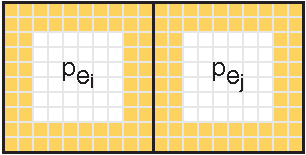
\includegraphics[height=.15\textheight]{images/pattern_interp.pdf}
    \caption{Material parameters in the border fine cells (orange) interpolate
    between coarse cell parameters $p_{e_i} \ne p_{e_j}$.}
    \label{fig:interpolate}
\end{figure}

Of course, it can happen that there is still a large jump in material parameters
after smoothing. This will lead to patterns that either cannot connect or that
are highly distorted. We will need to evaluate what happens here.

\subsection{Sequential Laminates}
Another approach is specific to the sequential laminate patterns, for which the
parameters are the material proportions and orientations for each of the $p$
lamination directions. There are two ways of going about this.
Recall that the lamination direction, $e_i$, as defined in
\cite{allaire2002shape} is a vector specifying the normal for the planar
lamination ``slices'' of material (see Figure \ref{fig:sequential_laminate}).
\begin{figure}[h!]
    \centering
    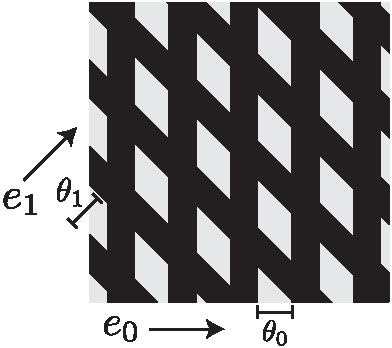
\includegraphics[height=.3\textwidth]{images/sequential_laminates.pdf}
    \caption{A sequential laminate is formed by iteratively laying down slices
        of a material of a particular width, $1 - \theta$, along a particular
    direction, $e$.}
    \label{fig:sequential_laminate}
\end{figure}

\subsubsection{Trace Lamination Directions}
\label{sec:direction_trace}
First, we could lay down slices perpendicularly to smooth lamination direction
curves fit to the direction vectors sitting on each element $e \in \mesh_c$.
These lamination direction curves
specify the line orthogonal to which thin planar slices of the material must be
added. We can also interpolate along each curve its associated $\theta$
parameter to determine the width of each slice. It is not immediately clear how
to choose the depth and height of each slice, nor how it will intersect with
neighboring planes. Also, it will be necessary to have many nearly uniformly
spaced lamination curves passing through each coarse element. We can attempt
this by seeding curves a specified distance away from existing ones and tracing
them until they either come too close or stray too far.

\subsubsection{Trace ``Dual'' Directions}
\label{sec:dual_trace}
Second, we could place holes along a different lamination direction curve: dual
edges of the lamination lattice. Notice that the voids/regions of weak material
in Figure \ref{fig:sequential_laminate} are all identical polygonal regions. In
general, sequential laminates generate a repeating grid of polyhedral holes. If
we can construct curves that form intersections only at the centers of
these holes, then we can synthesize the microstructure geometry by simply placing
polygons/polyhedrons sized and shaped according to the $e_i$s and $\theta_i$s at
that point. These curves are \textbf{not} interpolants of the lamination
directions. This operation is well defined in $2D$ for $p = 2$ laminate
directions and will yield something like Figure \ref{fig:hole_place}. For higher
$p$, it is more difficult to define. Also, for higher dimension it will be
difficult to ensure the lines intersect properly. Finally, it is important the
curves are of roughly uniform density, so a similar seeding and tracing strategy
is needed to the one above.

\begin{figure}[h!]
    \centering
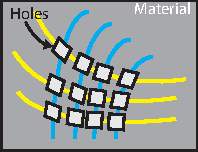
\includegraphics[height=0.3\textwidth]{images/hole_packing}
\caption{Illustration of the ``hole placing'' algorithm.}
\label{fig:hole_place}
\end{figure}

\subsubsection{Isosurface Synthesis}
\label{sec:isosurface}
Finally, we could take a more global approach analogous to crossfield-guided
parametrization: we could fit isosurface normals (isoline normals in
$2D$) of a scalar field, $f_i$, to each lamination direction, $e_i$, by solving
the Poisson equation. In energy form, this is:
$$
\min_{f_i} \sum_{i=1}^p \sum_{c \in \mesh_c} \norm{\nabla f_i - e_i(c)}^2.
$$
This will require a global labeling of lamination directions so that $e_i(c)$, the
$i^\text{th}$ direction on element $c$, is consistent with the $i^\text{th}$
direction of neighboring elements (see Section \ref{sec:registration}). This is
analogous to setting period jumps in Mixed Integer Quadrangulation.

Since each lamination direction is a unit vector, evenly
spaced isovalues will correspond to nearly evenly spaced isosurfaces.
Once a spacing is chosen, these isosurfaces can be extruded into lamination
slices with width depending on $\theta_i(x)$ (an interpolant of $\theta_i(e)$).

Notice that that Poisson solve effectively projects out the divergence-free
component of $e_i(c)$. If the direction fields have high curl, this approach
will not be able to accurately synthesize the laminate.

\subsubsection{Registration of Lamination Directions}
\label{sec:registration}
In $3D$, there will be $p \ge 3$ direction vectors in arbitrary
(non-orthogonal) orientation at each element. For all of these synthesis
approaches, it is important that we know which vectors are meant to connect to
which across elements. The material fitting algorithm assigns a label $e_i$ to
each direction, but our discrete laminate pattern is invariant to this labeling;
the lamination operation is a union of the slices and order does not matter.
(Beware that the formulas in \cite{allaire2002shape} are order-dependent and we
must figure out why). Since swapping the labeling of the $e_i$ yields the same
synthesized pattern at each point, we should compute the optimal matching of
labels between elements to minimize total direction deviations. This matching is
done either locally when tracing between a single pair of elements or globally
at the start (as needed for the isosurface synthesis approach). This ensures
that the pattern we synthesize changes minimally as it interpolates between
elements.

Even worse, for isotropic materials, the homogenized elasticity tensor is
invariant to a global rotation of the pattern. Thus, for the isotropic tensors,
we should solve for a rotation minimizing its deviation from its neighbors to
ensure the smoothest possible transitions.

Counterpoint: it is important to note that the input, thus the ground truth,
explicitly label lamination directions with $e_i$'s.  Apart from the isotropic
material case, the directions of lamination are well defined.  The only reason
for discarding the $e_i$ labeling, and thus justify the extra computation cost,
is if the labeling of $e_i$ could be inconsistent from point to point even for
non-isotropic target material.  This remains to be verified.

\subsection{Mesh Generation}
The procedure chosen for generating/connecting patterns must be
extended to stitch meshes together. E.g., for the general periodic pattern
connection approach described in Section \ref{sec:gen_connect}, identically
patterned neighboring cells can be stitched together trivially, and those with
similar boundary shapes could be stitched together after warping, assuming
consistent boundary meshing.

A procedural mesh generation must be defined for the procedures suggested
in Sections \ref{sec:direction_trace}, \ref{sec:dual_trace}, and
\ref{sec:isosurface}.

\subsection{Vertex Field Representation}
Although piecewise constant pattern parameters (and thus material tensors) are
simpler to use in computation, it is an unnecessary restriction when designing
microstructures.  After all, the target material properties are a smooth function
of the domain. Instead of piecewise constant, a piecewise trilinear
interpolation of the pattern parameters not only simplifies the tracing-based
sequential laminate synthesis approaches described in Sections
\ref{sec:direction_trace} and \ref{sec:dual_trace}, it also circumvents the need
of connecting microstructures between neighboring cells (Section
\ref{sec:general_periodic}).  This is because the lamination directions are
continuous across cell borders.  Furthermore, piecewise trilinear representation
could give a more accurate representation of the pattern parameters with fewer
elements. If the input pattern parameters are a per-element quantity, a
per-vertex quantity can always be obtained by interpolation.

Counterpoint:
The ground-truth, input elasticity tensors live on elements, and so our pipeline
first converts them into material properties that live on the elements.
Interpolating to per-vertex values is a somewhat arbitrary, mesh-dependent
approach to smoothing, though it does simplify the tracing-based approaches. A
smoothing/fitting technique on the original per-element data can be made more
accurate/smooth if needed. Furthermore, since our ground truth elasticity
tensors are on the tets, interpolating to per-vertex pattern parameters
introduces a quantitative error even if could give qualitatively better
behavior. Note that for the isosurface extrusion approach to discrete laminate
synthesis, the direction parameters must live on the elements. Finally,
per-coarse-vertex parameters \textbf{do not} get around warping microstructures
in Section \ref{sec:general_periodic} since we still use piecewise-constant
patterns on the fine cells to assign the fine cell geometry. It just replaces
the interpolation step mentioned there with a new one where each fine cell
differs from its neighbors in a trilinear way (as opposed to a scheme that
could be tuned and localized to the coarse boundary).

\section{Printability}
Not only do we need to choose the periodic cell size large enough that the
printer can resolve the patterns' details without violating any design rules,
but also we must worry about internal voids in the case of the single material
application. In the single material case, the patterns comprise solid and void
regions (as opposed to solid regions of distinct materials for multi-material
printing). To allow support material removal, these voids must all have a path
to the object's exterior.

The printibility concerns could be avoided when printing with multi-material
printers, where one can replace void with a very weak material.

\section{Search for Patterns}
It will be desirable to have periodic patterns that are
parametrized smoothly to allow stitching. Ideally these patterns will have
an analytic formula for their homogenized elasticity tensors/material
properties, but we may be able to get away with the numerical coarsening +
look-up-table-only fitting approach. It would also be nice if there are
well-defined direction parameters (as is the case with sequential laminates) to
enable the tracing/isosurface extrusion approaches.

Even more importantly, the pattern we choose must have good coverage of the
range of desired material properties. We discuss this in the next section.

\section{Toward a Proof of Concept}
The most important preliminary experiment is to test that we
can achieve a useful range of material properties with a single material
printer. The best tool we have for this is currently the sequential laminate
\cite{allaire2002shape}, since this gives us several closed formulas for
homogenized elasticity tensors. Perhaps other patterns can achieve a wider range
of materials, but we would need to develop our own machinery to analyze them.

So far we have looked only at the space of approximately isotropic homogenized
tensors achieved by rank $1, 2, $ and $3$ sequential laminates of two
non-void, isotropic materials. Though we have not analyzed all our data, we
found that the laminates were roughly able to interpolate between the two
materials' Young's moduli (Poisson ratio remained mostly unchanged). It will be
important to look also at the space of orthotropic materials. We also need to
consider the case were one material is void (Section 2.3.4 of
\cite{allaire2002shape}).


\section{Miscellaneous Concerns}
\begin{itemize}
    \item The homogenization theory is built around linear elasticity. If we want to
        design large-scale deformation behavior, we will probably have to
        consider a non-linear version (if possible).

    \item What material will be used to form the object's surface? It is likely
        that printing the skin will introduce rigidity that prevents all the
        deformation behavior our internal microstructures are designed to
        support.
\end{itemize}

\section{Implementation}
This section summarizes the all sections above in terms of work.

\subsection{Software}
The software would consist two independent modules:
\begin{description}
\item{\bf Convert arbitrary material tensor into pattern parameters}\\
{\it Input:} An array of material tensors.

{\it Output:} An array of pattern parameters (and fitting errors).\\

Approach 1: look up table.
\begin{itemize}
\item For microstructure with closed formula of homogenized material properties,
sample the space of all possible pattern parameter combinations.
\item For microstructure without closed formula of homogenized material
properties, use representative volume method to find it out.  I.e. For all
possible pattern parameters, generate a
cube made of microstructures, simulate it either on a very fine mesh, or use
Mesh-free techniques, or use \cite{Kharevych2009} to obtain the homogenized
material property.
\item For each sampled pattern parameter, compute the homogenized material
tensor.
\item Build a table that support fast lookup with material tensor as key.  If
the tensor is not in the table, return the closest entry using a reasonable
measure.
\end{itemize}

Approach 2: optimization of material parameters.



\item{\bf Generate microstructure geometry}\\
{\it Input:} An array of pattern parameters.

{\it Output:} Microstructure mesh


\end{description}

\subsection{Experiments}
Due to the slow turn around time, we have to plan ahead.

\section{Examples and experiments}
This section discribes the possible examples to include in the paper.
\begin{description}
\item{\bf Visually verifiable examples:}\\
This set of examples are mostly used for validation purposes where the expected
behavior is obvious.  For example, 
\begin{itemize}
    \item Rectangular bar of isotropic material with Young's modulus varying from one end
        to the other.
    \item Rectangular bar of orthotropic material with material axis rotating
        from one end to the other.
    \item A thin bar of various material properties such that when pinching both
    ends it deform in a zig-zag pattern instead of normal buckling. See Figure
    \ref{fig:zig_zag_bar}.
\end{itemize}
\begin{figure}
\centering
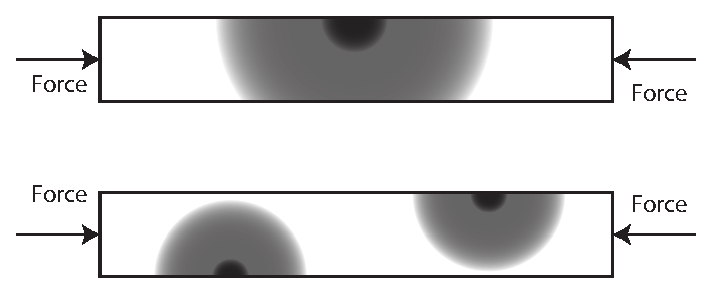
\includegraphics[width=0.5\textwidth]{images/zig_zag_bar}
\caption{White represent stronger material properties and black represent weaker
material properties.  One can achieve different bending behavior using the
material property specificaiton above.  Top: center kink.  Bottom: Zig-zag
deformation.}
\label{fig:zig_zag_bar}
\end{figure}

\item{\bf Compare with ``Design and Fabrication of Materials with Desired
Deformation Behavior'' \cite{Bickel2010}:}\\
The goal of comparing to \cite{Bickel2010} is to show the resulting
microstructure of our approach can approximate material properties of their
layered design.  For example, we could simulate poking the slipper sol (see
their teaser) twice: once with their sol design, and once with our
microstructure pattern.  Ideally both simulations yield the same displacements
of the poking location.

\item{\bf Compare with shape/topological optimization:}\\
As pointed out in \cite{allaire2002shape} \S 4.1.2, in compliance minimization
setting, the true optimal shape configuration under a given load is given by
microstructures.  Due to the complexity of the microstructures, one often need
to change the problem to get a quasi-optimal solution (ressembles truss
networks) that can be manufactured.  Since 3D printing, especially
multi-material printers, is agnostic about complexity, we could produce shapes
with microstrcuture that is stronger than truss networks.

\begin{figure}
\centering
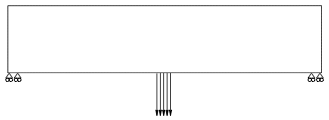
\includegraphics[width=0.5\textwidth]{images/3pt_bending}\\
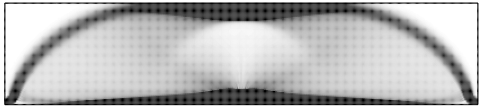
\includegraphics[width=0.5\textwidth]{images/micro_struct_bridge}\\
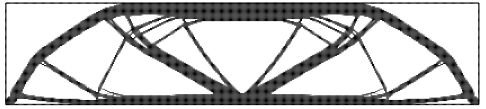
\includegraphics[width=0.5\textwidth]{images/truss_network_bridge}\\
\caption{Top: 3-point bending setup.  Middle: optimal microstructure.  The gray
region corresponds to microstructures.  Bottom:
quasi-optimal truss network.  Images taken from \cite{allaire1996homogenization}}
\label{fig:3pt_bending}
\end{figure}

As illustrated in Figure \ref{fig:3pt_bending}, we could print both the
microstructure bridge and the truss network bridge (note that both vertions uses
the same amount of material).  Subject both prints under center load and verify
the microstructure bidge is indeed stronger.  The micromaterial parameter is
part of the output of shape optimization in \cite{allaire1996homogenization}
(TODO: double check with Bob Kohn).

\item{\bf Compare with ``Computational Design of Actuated Deformable
Characters''
\cite{Skouras:2013}:}\\
One of the more practical applications is to print toy characters that can be
deformed into target poses.  In contrast to \cite{Skouras:2013}, our approach
can achieve the same effect with a single material.
(TODO: how to generate desired material tensors.)

\item{\bf Weight differentiator:}\\
This example aims to motivate real time applications of our work.  With
microstructure, one can achieve some cool nonlinear deformation effects. Figure
\ref{fig:weight_differentiator} illustrates the desire material properties for
building a simple ``weight differentiator''.  In particular, when the devise is
subject to small load, the top surface tilts leftward.  When the load is large,
the top surface tilts rightward.  This allow one to partition balls by weight
(e.g. drop a ball on it and the ball would bounce to the either left or right
depending on its weight).

\begin{figure}
\centering
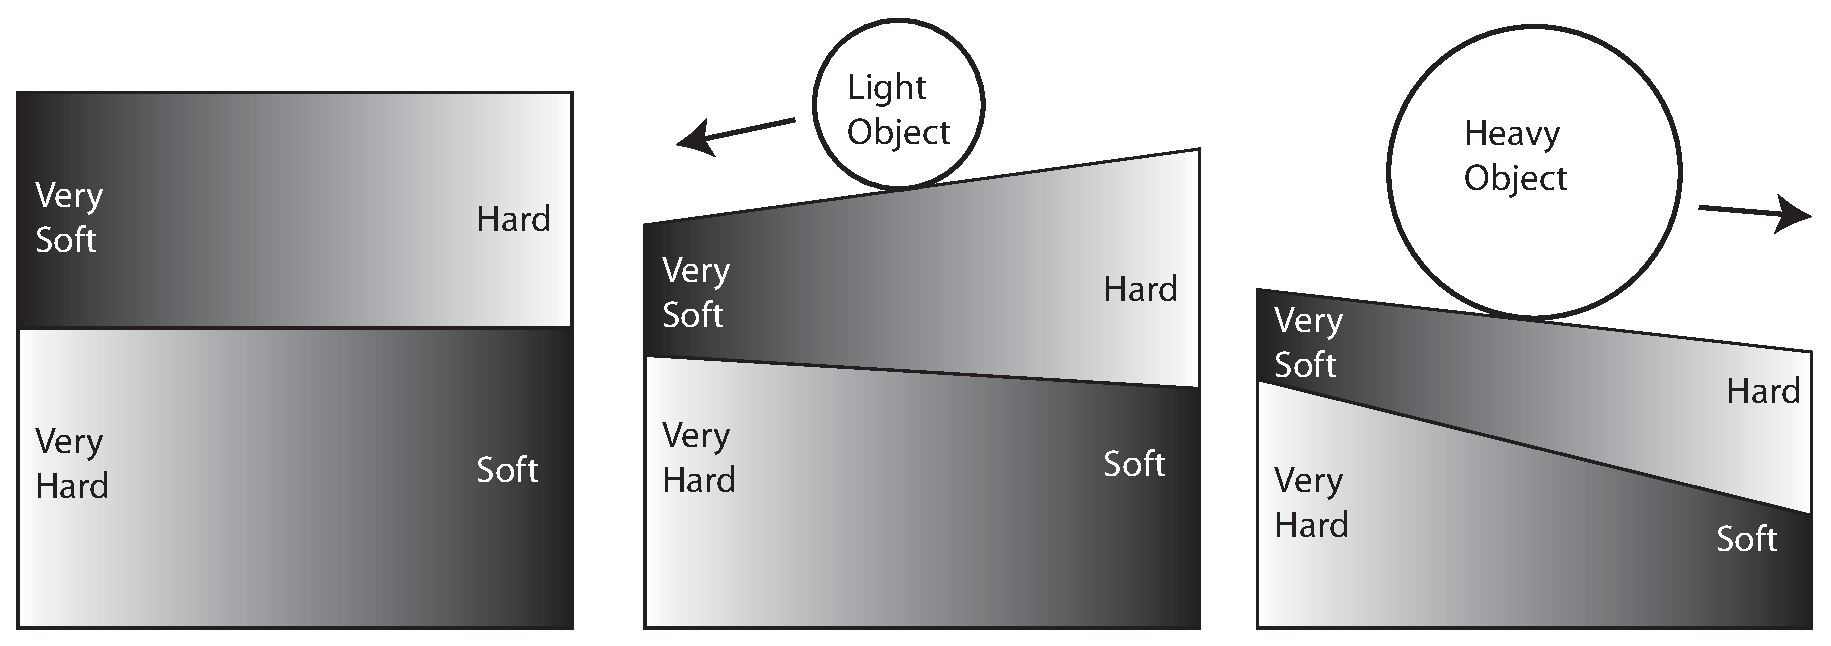
\includegraphics[width=0.9\textwidth]{images/weight_differentiator}
\caption{
Weight differentiator design is a purely static mechanical device to distinguish balls
with weight above or below a certain threshold.
Left: material specification of a cube.  Middle: under light
compressive force, the top surface tilts leftward.  Right: under heavy
compressive force, the top surface tilts rightward.}
\label{fig:weight_differentiator}
\end{figure}

\end{description}

Besides the examples above, we would need to carry out physical experiments to
validate the material properties of microstructures.  Here are the proposed
experiments:

\begin{description}
\item{\bf Material properties of the base material:}\\
We need to determine the material properties of our base material.

\item{\bf Validate sequential lamination formula:}\\
Specifically, validate equation 2.64 (p. 127) for rank-1 laminates, 2.67 for
rank-2 and 3 laminates and 2.151 (p. 167) in \cite{allaire2002shape}.  The
experiment would be 3-point bending test of perfectly tiled microstructures.
For microstructure of various refinements, we apply center load on it and record
the corresponding displacements.  Under infinite microstructure refinement, the
extrapolated displacement should be near the output of the formulas.

\item{\bf Validate algorithm described in section \ref{sec:gen_connect}:}\\
For most shapes, we won't be able to tile our pattern perfectly.  Thus an
experiment validation would be necessary to test whichever algorithm we choose to
generate the microstructures.  Again, 3 point bending test described above could
be used.  In this case, the samples should contain microstructure that is not
perfectly tiled (e.g. the bar in Figure \ref{fig:zig_zag_bar}).

\end{description}



\bibliographystyle{plain}
\bibliography{References}

\end{document}

